% =====================================================
\chapter{Experiments on Existing Solutions}
\label{chap:existing_solutions}

\noindent
Before evaluating any existing style-aware diffusion systems, a focused dataset was curated to represent the kind of distribution shifts observed in the wild.  
Approximately \textbf{500 images} were handpicked from publicly available sources such as Pinterest~\cite{pinterest}, iStock~\cite{istock}, and Google Images~\cite{google_images}, spanning a wide range of adverse environmental conditions such as fog, smog, heavy rain, snow, blizzard, sandstorm, dust storm, storm, and forest fire.  
These scenes were specifically selected because both the background and foreground elements are often veiled under a strong stylistic “shroud,” which makes object boundaries ambiguous and significantly complicates classification and detection tasks.  
This dataset serves as the common evaluation ground for all subsequent models.

\noindent
\textbf{Note:} Although testing and benchmarking were carried out across all environmental domains mentioned above, the following visual comparisons and analyses focus specifically on the \textbf{agriculture domain}, which was found to most effectively resonate with the objectives of realistic distribution-shift representation and volumetric environmental stylization.

\begin{figure}[!h]
    \centering
    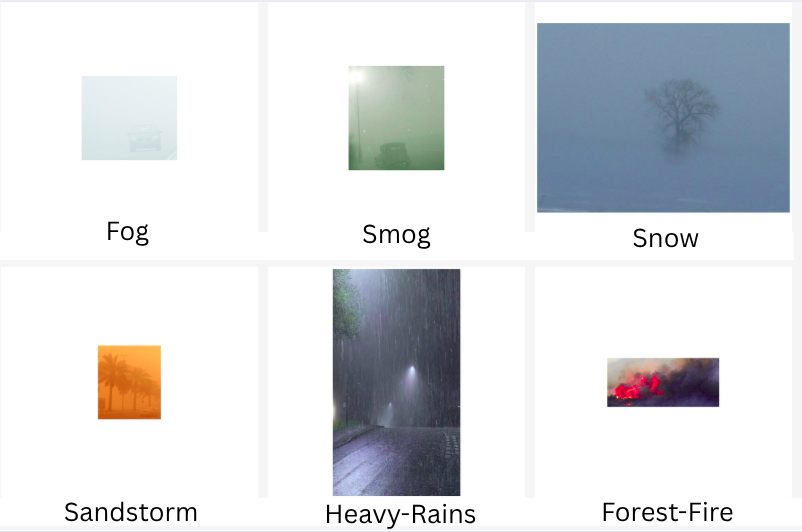
\includegraphics[width=\linewidth]{images/curated_dataset_collage.png}
    \caption{Representative collage from the curated dataset used for evaluation, spanning diverse environmental conditions such as fog, smog, snow, sandstorm, and forest fire. The agriculture domain subset (shown here) was selected for focused visual analysis due to its strong correspondence with real-world visibility and scattering effects.}
    \label{fig:curated_dataset_collage}
\end{figure}


% =====================================================
\section{StyleShot: One-Shot Style Transfer with Attention Modulation}
\label{sec:styleshot}

To explore prompt-guided, reference-based style transfer under environmental distribution shifts, the first existing solution evaluated was \textbf{StyleShot}~\cite{gao2024styleshot}.  
The experiments were carried out on the curated dataset mentioned above.  
These scenes were selected to intentionally represent the loss of visibility and structural ambiguity typical of style-induced distribution shifts, where both the background and foreground appear enveloped in a dense “style shroud.”  
The goal was to examine whether the model could convincingly reproduce such styles while maintaining semantic coherence.

\paragraph{Architecture Overview}
As illustrated in Figure~\ref{fig:styleshot_architecture}, the original StyleShot framework is designed as a \textbf{tri-modal diffusion system}, integrating three modalities: text, content, and style into a unified diffusion backbone.  
It consists of three encoders:  
(1) a \textbf{Style-Aware Encoder} that partitions the style reference image into multiple scales and embeds each partition using transformer blocks (OpenCLIP ViT-H/14)~\cite{radford2021clip} to capture tone, color, and texture statistics;  
(2) a \textbf{Content-Fusion Encoder} that processes edge maps or structure references to maintain spatial layout  and  
(3) a \textbf{CLIP Text Encoder} that provides semantic grounding for prompt-based control.  
These embeddings are fused within the diffusion U–Net~\cite{ronneberger2015unet} via \textbf{Parallel Cross-Attention} and \textbf{Residual Addition}, enabling the network to modulate appearance (from the style image) while preserving textual and structural semantics~.

\begin{figure}[!h]
    \centering
    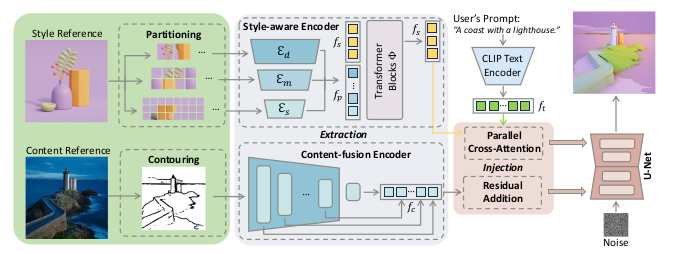
\includegraphics[width=0.75\linewidth]{images/styleshot_architecture.png}
    \caption{Overall architecture of StyleShot~\cite{gao2024styleshot}: tri-modal fusion of style, content, and text embeddings through parallel cross-attention and residual addition in the diffusion U–Net.}
    \label{fig:styleshot_architecture}
\end{figure}

\paragraph{Modified Experimental Configuration}
In this work, the setup was simplified to reflect the \textbf{text + style reference} configuration, as the curated dataset did not include explicit content reference images or edge maps.  
Accordingly, the \textit{Content-Fusion Encoder} branch was disabled.  
The model thus operated as a \textbf{bi-modal diffusion system}, driven by the CLIP text embeddings for semantic composition and the style-aware embeddings for texture and tone modulation.  
While the paper depicts the full tri-modal fusion (Figure~\ref{fig:styleshot_architecture}), in our experimental setting only the \textit{Style-Aware Encoder} and \textit{CLIP Text Encoder} contributed to conditioning.  
The fusion occurred through parallel cross-attention layers within the diffusion U–Net, where style tokens (\(f_s\)) and text embeddings (\(f_t\)) jointly influenced the denoising trajectory:
\[
\text{Attn}_{\text{final}} = \text{Attn}(Q, K_t, V_t) + \lambda_s \, \text{Attn}(Q, K_s, V_s),
\]
with \(\lambda_s\) controlling the relative style strength.  
This configuration aligns with the objectives of this study, which involve text-driven style transfer under distribution shift, where the style reference image represents an environmental condition such as haze, snow, or dust.

\paragraph{Results}
When evaluated on the curated dataset, StyleShot~\cite{gao2024styleshot} generated outputs that were visually rich but \textbf{overly artistic} and aesthetically biased rather than physically realistic.  
The model often prioritized stylistic exaggeration over faithful reconstruction, producing textures reminiscent of oil painting or digital art.  
This deficiency became evident in agricultural and outdoor scenes, where machinery and terrain edges remained sharply defined while the background appeared painterly and abstract.  
Similarly, in underwater or snow-heavy conditions, StyleShot was unable to simulate realistic scattering, depth-based attenuation, or backscatter, producing flattened tones that lacked the characteristic bluish-green absorption seen in real imagery.  

\begin{figure}[!h]
    \centering
    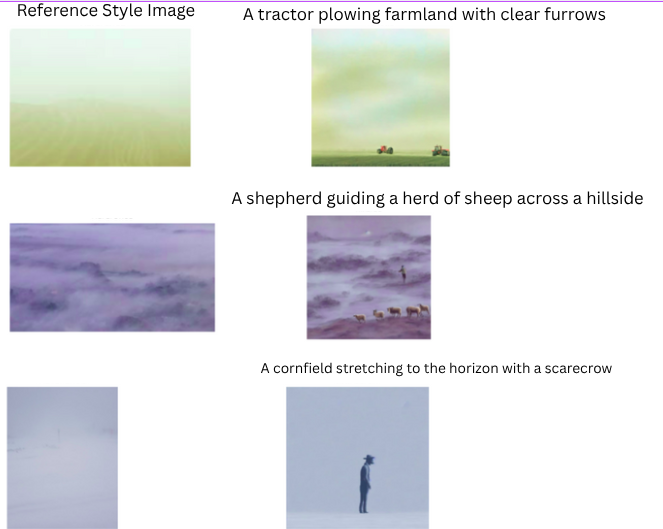
\includegraphics[width=0.85\linewidth]{images/styleshot_fail_agriculture.png}
    \caption{StyleShot on curated agricultural scenes: over-stylization and lack of depth-consistent haze. Foreground regions remain overly sharp while the background becomes painterly.}
    \label{fig:styleshot_fail_agri}
\end{figure}

\paragraph{Inference}
StyleShot offers an elegant and training-free mechanism for reference-based style transfer but demonstrates clear limitations when applied to environmental domain adaptation tasks.  
Its diffusion outputs are dominated by artistic stylization, fail to produce realistic haze or scattering around the foreground, and often degrade structural fidelity.  
These shortcomings motivate the exploration of more adaptive, physics-aware frameworks such as InstantStyle~\cite{wang2024instantstyle}, CSGO~\cite{xing2024csgocomp}, and the proposed CSD~\cite{somepalli2024csd} guided approach in later sections.

% =====================================================
\section{CSGO: Content–Style Composition in Text-to-Image Generation}
\label{sec:csgo}

To assess an end-to-end trained alternative to tuning-free stylization, we evaluated \textbf{CSGO (Content–Style Composition)~\cite{xing2024csgocomp}} on the curated extreme-conditions set. The objective remains to transfer the environmental “style shroud” while preserving scene semantics and producing physically plausible depth-dependent effects.

\paragraph{Architecture Overview and Configuration}
CSGO is built on an SDXL backbone~\cite{podell2023sdxl} and explicitly \emph{decouples} content and style controls.  
A \emph{content pathway} injects CLIP image encoder features~\cite{radford2021clip} via cross-attention in the down blocks and a \emph{Tile ControlNet} stream~\cite{zhang2023controlnet} in the up blocks.  
In parallel, a \emph{style pathway} encodes the reference style image using a ViT-H encoder~\cite{dosovitskiy2020vit} and a Perceiver Resampler, injecting tokens into both the U–Net and ControlNet.  
Training uses the \textbf{IMAGStyle} dataset (210k triplets) with content from MSRA10K/MSRA-B and styles from WikiArt and Midjourney.
\begin{figure}[!h]
    \centering
    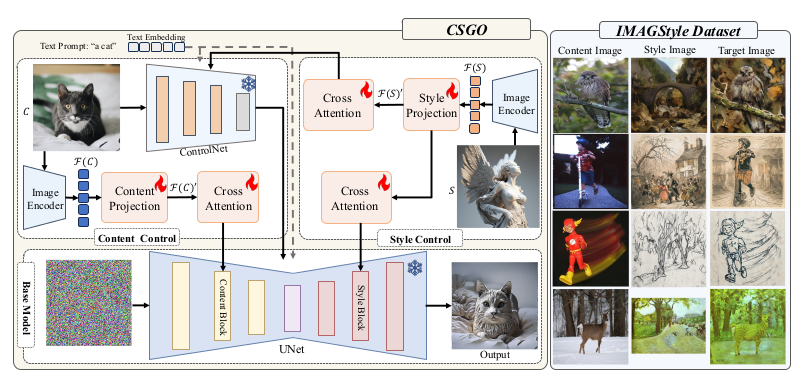
\includegraphics[width=0.75\linewidth]{images/csgo_architecture.png}
    \caption{Overview of the CSGO framework: decoupled content and style pathways fused into SDXL with ControlNet support (adapted from Xing et al., 2024~\cite{xing2024csgocomp}).}
    \label{fig:csgo_architecture}
\end{figure}

In this study, CSGO was run in a \textbf{text + style} regime (no content reference).  
A blank canvas was provided as content input; prompts defined semantics, and the style image supplied appearance tokens.  
ControlNet (Tile) was used at low conditioning scale (0.2).  
Sampling used 50 steps, guidance 5.5, \texttt{style\_scale}=1.0, \texttt{content\_scale}=1.3.

\paragraph{Results}
CSGO delivered strong stylistic color bias but lacked physics-consistent environmental haze.  
Foregrounds stayed sharp while backgrounds were softly recolored, failing to create volumetric occlusion.  
Underwater and fog scenes lacked depth-dependent attenuation and scattering, producing flatter results.

\begin{figure}[!h]
    \centering
    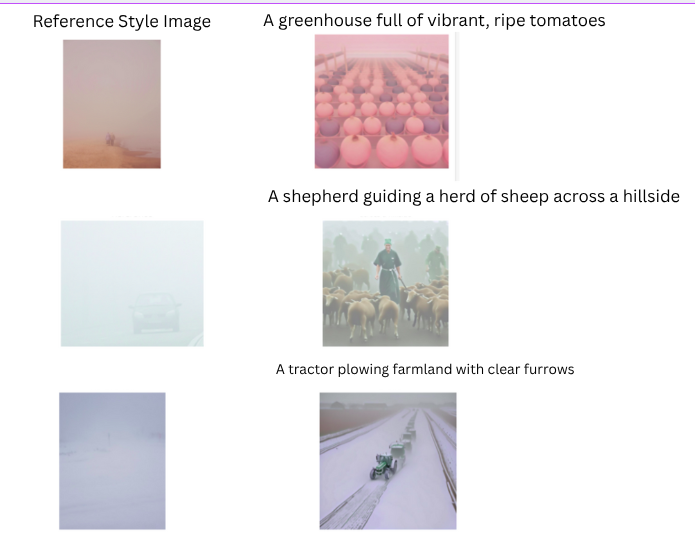
\includegraphics[width=0.85\linewidth]{images/csgo_fail_agriculture.png}
    \caption{CSGO on curated agricultural scenes (text+style setup): texture transfer without depth-consistent haze; crisp foreground edges.}
    \label{fig:csgo_fail_agri}
\end{figure}

\paragraph{Inference}
CSGO provides a solid framework for content–style separation but, in a text+style setup, lacks physical realism.  
Without a content image prior or strong ControlNet, style behaves like recoloring rather than volumetric shrouding.  
This motivates physics-aware guidance in later models.


% =====================================================
\section{InstantStyle: Style-Preserving Injection with IP-Adapter}
\label{sec:instantstyle}

Among all evaluated methods, \textbf{InstantStyle}~\cite{wang2024instantstyle} consistently delivered physically grounded and semantically coherent text-guided style transfer across adverse environmental domains.  
As a tuning-free adapter-based framework built on SDXL~\cite{podell2023sdxl}, it introduced a minimalist yet powerful mechanism for injecting style residuals directly into the diffusion process without modifying the base network weights.  
This approach offered the best trade-off between \textit{semantic consistency, structural fidelity}, and \textit{visual realism}, setting the stage for adaptive variants such as InstantStyle-Plus~\cite{wang2024instantstyleplus}.

\paragraph{Architecture and Embedding Formulation}
InstantStyle augments the SDXL backbone with an additional \textit{Image Prompt Adapter} (IP-Adapter~\cite{chen2023ipadapter}) that encodes the style image in the same latent CLIP~\cite{radford2021clip} space as the text embedding.  
Given a text prompt \( t \) and a style image \( I_s \), the system computes the following CLIP embeddings:
\[
\mathbf{e}_t = f_{\text{text}}(t), \qquad
\mathbf{e}_s = f_{\text{img}}(I_s),
\]
where \( f_{\text{text}}(\cdot) \) and \( f_{\text{img}}(\cdot) \) denote the text and image encoders of the pre-trained CLIP model respectively.  
To disentangle appearance from semantics, InstantStyle applies a simple but effective subtraction in the CLIP feature space:
\[
\mathbf{e}_{\text{style}} = \mathbf{e}_s - \beta \, \mathbf{e}_t,
\]
where \( \beta \) is a scaling coefficient (typically \( \beta \in [0.6,0.8] \)) controlling the degree of content suppression.  
This residual embedding \( \mathbf{e}_{\text{style}} \) encodes pure stylistic cues—color palette, illumination, texture statistics—while discarding semantic overlap with the text description.

The resulting style tokens are linearly projected into the attention space of SDXL’s U–Net~\cite{ronneberger2015unet} via the IP-Adapter, forming a set of key–value pairs:
\[
(\mathbf{K}_{\text{style}}, \mathbf{V}_{\text{style}}) = \mathcal{P}(\mathbf{e}_{\text{style}}),
\]
where \( \mathcal{P}(\cdot) \) denotes the learned style projection module.  
These pairs are injected into selected mid- and up-block cross-attention layers, replacing or complementing the text-based conditioning.  
Thus, for an intermediate latent feature \( \mathbf{z}_l \) at layer \( l \), the attention update becomes:
\[
\mathrm{Attn}_l(\mathbf{z}_l)
= \mathrm{softmax}\!\left(\frac{\mathbf{Q}_l \, [\mathbf{K}_t \, \| \, \mathbf{K}_{\text{style}}]^{\!\top}}{\sqrt{d}}\right)
[\mathbf{V}_t \, \| \, \mathbf{V}_{\text{style}}],
\]
where \( \| \) denotes concatenation along the token dimension, ensuring that both semantic and stylistic contexts influence the generative trajectory.

\begin{figure}[!h]
    \centering
    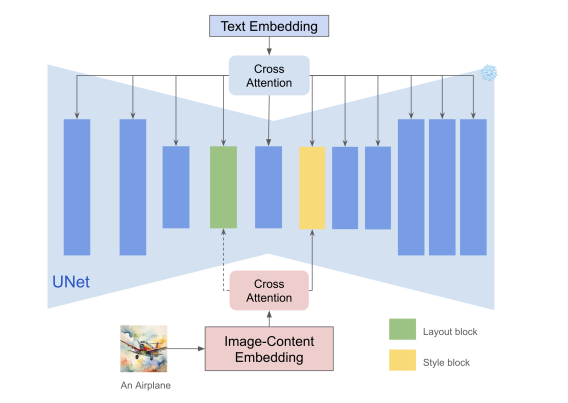
\includegraphics[width=0.7\linewidth]{images/instantstyle_architecture.png}
    \caption{InstantStyle architecture: CLIP-based text and style embeddings, residual subtraction, and IP-Adapter cross-attention injection into SDXL layers (adapted from Wang et al., 2024~\cite{wang2024instantstyle}).}
    \label{fig:instantstyle_architecture}
\end{figure}

\paragraph{Configuration and Modes}
We evaluated two principal modes:
\begin{itemize}
    \item \textbf{Soft Mode:} 40 diffusion steps, guidance 6.8, and style scale 0.83 — prioritizing volumetric realism and semantic faithfulness.
    \item \textbf{Strong Mode:} Higher guidance and style scale, emphasizing contrast and saturation at the expense of depth consistency.
\end{itemize}

Additionally, a \textbf{tuned-soft} variant relaxed anti-blur terms in the negative prompt, such as “sharp focus” and “deformed,” to allow physically consistent diffusion of light and haze in weathered environments.

\paragraph{Results}
Across the agriculture domain, InstantStyle’s tuned-soft configuration produced perceptually rich and physically consistent results.  
The model achieved volumetric haze and subtle scattering effects while retaining the structural geometry of the base content.  
Foreground objects remained coherent with the background illumination, demonstrating the framework’s ability to generalize to unseen distributions without explicit retraining.

\begin{figure}[!h]
    \centering
    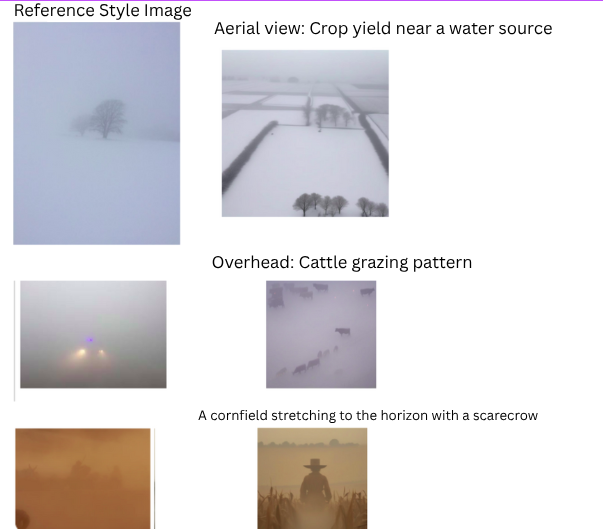
\includegraphics[width=0.65\linewidth]{images/instantstyle_results.png}
    \caption{InstantStyle results on the agriculture benchmark: the tuned-soft variant maintains volumetric realism and illumination consistency; strong mode exaggerates stylization.}
    \label{fig:instantstyle_results}
\end{figure}


\paragraph{Inference}
The InstantStyle pipeline achieved efficient inference (typically under 8\,GB GPU memory for \(896\times896\) resolution) and remained stable across varied lighting and atmospheric conditions.  
Its explicit CLIP-space decomposition and attention-layer style fusion provided controlled, interpretable stylization without the instability often observed in ControlNet systems.

\paragraph{Summary}
InstantStyle thus serves as the \textbf{foundational bridge} between appearance injection and semantic conditioning under environmental distribution shift.  
While StyleShot offered aesthetic coherence and CSGO achieved explicit disentanglement, only InstantStyle reached a consistent equilibrium between physical plausibility and semantic precision.  
This balance motivated its natural evolution into \textbf{InstantStyle-Plus~\cite{wang2024instantstyleplus}}, where ControlNet~\cite{zhang2023controlnet} spatial priors and CSD~\cite{somepalli2024csd}-guided perceptual constraints extend the architecture toward adaptive, context-aware diffusion.


% =====================================================
% \section{Summary}
% \label{sec:existing_summary}

% StyleShot produced aesthetic but non-physical results, CSGO provided structured disentanglement but lacked volumetric realism, and InstantStyle achieved balanced, physically grounded stylization.  
% The tuned-soft InstantStyle run proved most effective, motivating further extensions such as \textbf{InstantStyle-Plus} and \textbf{CSD-Guided Diffusion} for controlled, environment-aware adaptation.
